We evaluate three questions. RQ1 measures compressed-file reduction and the records
retained for preservation. RQ2 measures cleanup time, memory and total
cleanup-plus-opening time. RQ3 tests structural preservation and Excel-rendered
appearance within the stated validation scope.

\subsection{Corpus identity and outcome accounting}
Data.gov, Destatis and Enron are evaluated separately. Archive checksums, member
names and duplicate occurrences identify each corpus version. XLS conversion is
reported separately from XLSX cleanup. Recursive extraction of Internet Archive's
EDRM Enron v2 XML archives inspected nested archives and embedded containers. It
yielded 34,065 distinct SHA-256-addressed candidates, including legacy Excel files
and other OLE objects. The prepared Enron XLSX evaluation population is described
below.

For native visual stress tests, we select the 49 workbooks with the largest
absolute compressed-file reduction from each corpus, totaling 147 original
identities. Every processor baseline uses these identities. Preparation, cleanup
and visual comparison have separate outcome counts.

The frozen XLSX inventories contain 9,117 Data.gov members totaling 25.273 GB and
1,182 Destatis members totaling 2.364 GB, measured as compressed file bytes in
decimal GB. Each member has a SHA-256 identity. Outcomes distinguish completed
comparisons, differences, failures, unsupported formats and unfinished work.
Retries are counted separately. Identical packages can bypass visual comparison.
Failed captures cannot establish equality.

\subsection{Cleanup screening outcomes}
Fresh release-build runs produced 1,182 Destatis, 8,623 Data.gov, and 30,301
prepared Enron XLSX outputs. Across those outputs, aggregate compressed
file bytes fell by 15.48\%, 5.27\%, and 18.87\%, respectively.
The smaller, equal-size, and larger output counts were
1,045/30/107 for Destatis, 4,755/3,522/346 for Data.gov, and
21,565/8,415/321 for Enron. Hash checks confirmed byte identity for all
equal-size outputs in these runs. Data.gov also had 494 unsupported-namespace
skips. With sixteen workbook slots and sixteen Rayon threads, elapsed times
were 119.7, 1,134.5, and 181.6\,s, respectively, including analysis statistics
and full replay events alongside concurrent native validation~\cite{corpusdistributions}.
All three runs reached completion with zero reported processing failures.
The host used an AMD Ryzen 7 7800X3D with eight physical cores, sixteen logical
processors, 95.1\,GiB OS-visible RAM and Windows 11 Home build 26200.
Interactive replays accompany the
\href{https://alexander-aue-johr.github.io/excel-shrink-paper/replays/corpus-distributions-20261111/destatis/}{Destatis},
\href{https://alexander-aue-johr.github.io/excel-shrink-paper/replays/corpus-distributions-20261111/datagov/}{Data.gov}
and \href{https://alexander-aue-johr.github.io/excel-shrink-paper/replays/corpus-distributions-20261111/enron/}{prepared Enron XLSX}
runs; replay clocks additionally include final reporting.
Successful processing of these inputs does not establish correctness for every
valid serialization.
These descriptive results include files that grew and use only processed
input bytes as the denominator. Enron's denominator begins after
preparation. Visual preservation is evaluated separately.
Figure~\ref{fig:corpus-distributions} shows the workbook and worksheet
distributions for these runs. Empty-cell cleanup and trailing layout rows
account for prominent worksheet XML reductions. The contribution of column
range merging is especially visible in Destatis. The worksheet panels exclude
88 prepared Enron workbooks without worksheet XML observations. Workbook payload sizes use all uncompressed ZIP member sizes.
\begin{figure*}[t]
\centering
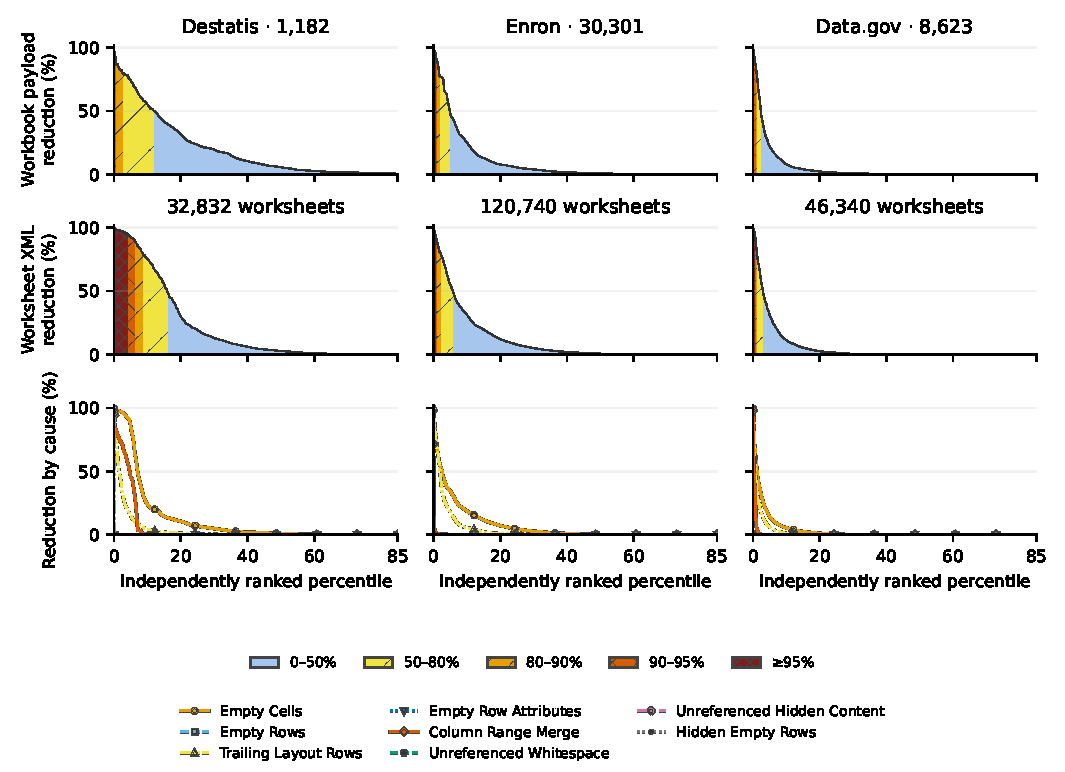
\includegraphics[width=\textwidth]{figures/corpus-uncompressed-distributions.pdf}
\caption{Full-corpus uncompressed-size reduction. Top, complete workbook
payload from all ZIP member sizes recorded in the central directory.
Middle, uncompressed worksheet XML.
Bottom, worksheet XML reduction attributed to each recorded cleanup cause.
Each curve independently sorts its observations from greatest to least
reduction. The x-axis gives the fraction of observations traversed in that
ordering. The common display ends at the 85th percentile. Remaining positive
reductions are below 0.5 percentage points. The omitted tail includes unchanged
outputs and growing workbooks (3/24/5) and worksheets (82/143/39), in
Destatis/Enron/Data.gov order, retained in the accompanying data.
Colors and hatching mark 50/80/90/95\% reduction tiers.
Data.gov's 494 unsupported-namespace
inputs are excluded from these processed-output distributions. The worksheet
panels cover 1,182 Destatis, 30,213 Enron and 8,623 Data.gov workbooks with
recorded worksheet XML. Enron begins with prepared XLSX inputs.}
\label{fig:corpus-distributions}
\end{figure*}

Among 9,117 Data.gov inputs, 493 workbooks contained explicitly prefixed
worksheet data elements. After experimental namespace normalization and Default
cleanup, only two produced smaller compressed packages, by 6.415\% and 0.047\%
relative to the normalized baseline. Cell-record removal in other outputs did
not reduce package size~\cite{prefixeddataexperiment}.

Corpus testing exposed parsing and preservation defects. Enron controls identified
missing center-across-selection spans and fill masks by restoring the affected
original cell records. These findings informed regression fixtures and native
Excel controls that complement the screening results~\cite{enrondefaultcontrols}.

\subsection{Sampling and reference controls}
We select the random sample from a frozen eligible population using a recorded
seed before inspecting visual results. Sampling strata reflect corpus, package
size and structural features known before validation. Low-reduction and unchanged
files remain included. A separately labelled development stress set contains large
and historically problematic workbooks.

Where feasible, sampled files receive full native reference captures of the
relevant visual area, independently of the candidate selector. Timeouts remain in
the denominator, without substituting easier workbooks. Test mutations introduce
known visible changes to values, styles, geometry, conditional dependencies and
objects. Changes normalized away by Excel are reported separately.

\subsection{Performance and comparison subjects}
We compared direct open--save trials with fresh six-worker SheetShrink cleanup
followed by the same library. Across the two displayed laptop workbooks, all 33 SheetShrink
trials completed under a 4\,GiB commit limit, compared with 21 original trials.
Median elapsed time improved in all seven fully completed pairs. Migration
with openpyxl took 111.3\,s directly and 9.7\,s including cleanup.

Tables~\ref{tab:case-study-transformations} and
\ref{tab:case-study-resources} join the opening/memory case study through frozen
file identities. The full experiment retains 288 opening/saving attempts
across six variants and three repetitions. The selected
Enron workbook has a separate eighteen-attempt follow-up on the larger-memory
host, described below. Its measurements retain their own host and configuration.
The tables display Migration and QT/RR, with Enron size evidence and a separate
resource follow-up.
The payload table uses exact retained comparator outputs and separately regenerated
Sheet Shrink controls with verified native-candidate member identities. Per-trial
member inventories of timed fresh outputs were not retained. Native pixel counts
are reported only for measured, retained image pairs with matched origins.
Missing scopes and image-size differences remain explicit.

The compact resource table reports total elapsed time and library working-set
peaks. The artifact separately retains pipeline working sets and job-commit
peaks. Each displayed time is a median of completed attempts,
with memory maxima over all three attempts. Stopped attempts retain their
elapsed time and memory boundary. Existing prepared-output
variants measure subsequent library processing. Fresh Sheet Shrink rows include
cleanup within the measured pipeline. The common host is a Ryzen 5 4500U laptop
with six logical processors, 8 GiB installed RAM and Windows 11. Each job has a
4 GiB commit cap and a 900 s timeout, with the free-RAM reserve disabled.
The Sheet Shrink executable is frozen at revision \texttt{765c480} and uses six
Rayon and six writer workers. Native visual observations use the retained
paired-rebuild protocol.

\begin{table*}[t]
\centering
\footnotesize
\setlength{\tabcolsep}{2.5pt}
\renewcommand{\arraystretch}{1.08}
\caption{Selected-case uncompressed payload reduction and retained native pixel evidence. Payload is the sum of all ZIP-member sizes in decimal MB. Image-pair counts state measured/recorded coverage.}
\label{tab:case-study-transformations}
\begin{tabular}{lrl}
\hline
Variant & Payload MB (reduction) & Changed / compared pixels; coverage \\
\hline
\multicolumn{3}{l}{\textbf{Destatis Migration}} \\
Original & \CasePairBars[4.4]{248.39 (0\%)}{1.09990}{1.09990}{casebarblue} & Reference \\
SheetShrink\textsuperscript{*} & \CasePairBars[4.4]{16.46 (93\%)}{1.09990}{0.07288}{casebarblue} & \begin{tabular}[c]{@{}l@{}}0 / 101,874,379\\37/38 image pairs\\5 size differences\\Normalized baseline\end{tabular} \\
NXPowerLite & \CasePairBars[4.4]{197.48 (20\%)}{1.09990}{0.87447}{casebarblue} & Failed \\
XLStylesTool & \CasePairBars[4.4]{248.42 (-0.0095\%)}{1.09990}{1.10000}{casebarorange} & Failed \\
Check Performance & \CasePairBars[4.4]{20.15 (92\%)}{1.09990}{0.08922}{casebarblue} & Memory limit \\
Inquire & \CasePairBars[4.4]{116.44 (53\%)}{1.09990}{0.51559}{casebarblue} & Failed \\
\hline
\multicolumn{3}{l}{\textbf{Data.gov QT/RR}} \\
Original & \CasePairBars[4.4]{1350.77 (0\%)}{1.10000}{1.10000}{casebarblue} & Reference \\
SheetShrink\textsuperscript{*} & \CasePairBars[4.4]{29.91 (98\%)}{1.10000}{0.02436}{casebarblue} & No capture regions \\
NXPowerLite & \CasePairBars[4.4]{29.98 (98\%)}{1.10000}{0.02442}{casebarblue} & No capture regions \\
XLStylesTool & \CasePairBars[4.4]{1350.77 (-7.8e-05\%)}{1.10000}{1.10000}{casebarorange} & No capture regions \\
Check Performance & \CasePairBars[4.4]{25.59 (98\%)}{1.10000}{0.02084}{casebarblue} & No capture regions \\
Inquire & \CasePairBars[4.4]{30.13 (98\%)}{1.10000}{0.02454}{casebarblue} & No completed report \\
\hline
\multicolumn{3}{l}{\textbf{Enron b2d0dfef}} \\
Original & \CasePairBars[4.4]{353.15 (0\%)}{1.09999}{1.09999}{casebarblue} & Reference \\
SheetShrink\textsuperscript{*} & \CasePairBars[4.4]{2.58 (99\%)}{1.09999}{0.00804}{casebarblue} & No retained pairs (0/2824) \\
NXPowerLite & \CasePairBars[4.4]{2.55 (99\%)}{1.09999}{0.00795}{casebarblue} & \begin{tabular}[c]{@{}l@{}}6,437 / 11,640,701,446\\1033/1033 image pairs\end{tabular} \\
XLStylesTool & \CasePairBars[4.4]{353.16 (-0.0011\%)}{1.09999}{1.10000}{casebarorange} & No capture regions \\
Check Performance & \CasePairBars[4.4]{2.54 (99\%)}{1.09999}{0.00792}{casebarblue} & \begin{tabular}[c]{@{}l@{}}456,503 / 46,890,576\\8/1032 image pairs\\2 size differences\end{tabular} \\
Inquire & \CasePairBars[4.4]{2.57 (99\%)}{1.09999}{0.00801}{casebarblue} & \begin{tabular}[c]{@{}l@{}}9,739 / 11,728,328,854\\1040/1040 image pairs\\1040 size differences\end{tabular} \\
\hline
\end{tabular}
\par\smallskip
\begin{minipage}{0.98\textwidth}\footnotesize \textsuperscript{*}SheetShrink uses separately regenerated controls whose uncompressed members match the native candidates; full per-trial member inventories of the timed pipelines were not retained. Wanderungen uses a normalized baseline. Counts compare exact RGBA values in common rectangles with matched origins; overlapping captures can count pixels repeatedly. Image-size differences remain separate from common-area pixel counts. Different plans and incomplete scopes preclude a cross-tool preservation ranking. No capture regions or retained pairs provide no pixel-equality observation. Gray bars show the original; blue/orange show payload at or below/above the original. Input/output hashes, scope details and failures remain in the artifact.\end{minipage}
\end{table*}

\begin{table*}[p]
\centering
\footnotesize
\setlength{\tabcolsep}{2.5pt}
\renewcommand{\arraystretch}{1.08}
\caption{Opening/saving observations on two hosts. Cells show median total seconds above maximum memory across three attempts. Host blocks specify commit caps and memory metrics. The timeout is 900 s.}
\label{tab:case-study-resources}
\begin{tabular}{lrrrrrr}
\hline
Endpoint & Original & SheetShrink & NXPowerLite & XLStylesTool & \shortstack{Check\\Performance} & Inquire \\
\multicolumn{7}{l}{\textbf{Ryzen 5 4500U laptop: 4 GiB commit cap; library working set (MiB)}} \\
\hline
\multicolumn{7}{l}{\textbf{Destatis Migration}} \\
openpyxl & \shortstack[r]{\CasePairBars[2.2]{111.30}{1.10000}{1.10000}{casebarblue}\\\CasePairBars[2.2]{2700}{1.09997}{1.09997}{casebarblue}} & \shortstack[r]{\CasePairBars[2.2]{9.67}{1.10000}{0.09555}{casebarblue}\\\CasePairBars[2.2]{250}{1.09997}{0.10194}{casebarblue}} & \shortstack[r]{\CasePairBars[2.2]{83.58}{1.10000}{0.82602}{casebarblue}\\\CasePairBars[2.2]{1996}{1.09997}{0.81334}{casebarblue}} & \shortstack[r]{\CasePairBars[2.2]{111.13}{1.10000}{1.09829}{casebarblue}\\\CasePairBars[2.2]{2700}{1.09997}{1.10000}{casebarorange}} & \shortstack[r]{\CasePairBars[2.2]{9.11}{1.10000}{0.09002}{casebarblue}\\\CasePairBars[2.2]{236}{1.09997}{0.09603}{casebarblue}} & \shortstack[r]{\CasePairBars[2.2]{54.96}{1.10000}{0.54318}{casebarblue}\\\CasePairBars[2.2]{1530}{1.09997}{0.62347}{casebarblue}} \\
pandas to XLSX & \shortstack[r]{\colorbox{caseadverse}{\strut M}\\3900} & \shortstack[r]{35.83\\856} & \shortstack[r]{\colorbox{caseadverse}{\strut M}\\3900} & \shortstack[r]{\colorbox{caseadverse}{\strut M}\\3900} & \shortstack[r]{\colorbox{caseadverse}{\strut M}\\3900} & \shortstack[r]{\colorbox{caseadverse}{\strut M}\\3900} \\
pandas to CSV & \shortstack[r]{\colorbox{caseadverse}{\strut M}\\3900} & \shortstack[r]{11.54\\214} & \shortstack[r]{\colorbox{caseadverse}{\strut M}\\3900} & \shortstack[r]{\colorbox{caseadverse}{\strut M}\\3900} & \shortstack[r]{\colorbox{caseadverse}{\strut M}\\3900} & \shortstack[r]{\colorbox{caseadverse}{\strut M}\\3900} \\
Excel COM & \shortstack[r]{\CasePairBars[2.2]{20.34}{1.10000}{1.10000}{casebarblue}\\\CasePairBars[2.2]{429}{1.10000}{1.10000}{casebarblue}} & \shortstack[r]{\CasePairBars[2.2]{9.92}{1.10000}{0.53635}{casebarblue}\\\CasePairBars[2.2]{309}{1.10000}{0.79239}{casebarblue}} & \shortstack[r]{\CasePairBars[2.2]{17.94}{1.10000}{0.96972}{casebarblue}\\\CasePairBars[2.2]{409}{1.10000}{1.04743}{casebarblue}} & \shortstack[r]{\CasePairBars[2.2]{20.17}{1.10000}{1.09070}{casebarblue}\\\CasePairBars[2.2]{428}{1.10000}{1.09743}{casebarblue}} & \shortstack[r]{\CasePairBars[2.2]{5.34}{1.10000}{0.28867}{casebarblue}\\\CasePairBars[2.2]{259}{1.10000}{0.66287}{casebarblue}} & \shortstack[r]{\CasePairBars[2.2]{9.99}{1.10000}{0.53998}{casebarblue}\\\CasePairBars[2.2]{324}{1.10000}{0.83184}{casebarblue}} \\
R openxlsx & \shortstack[r]{\CasePairBars[2.2]{44.38}{1.08690}{1.08690}{casebarblue}\\\CasePairBars[2.2]{824}{1.09028}{1.09028}{casebarblue}} & \shortstack[r]{\CasePairBars[2.2]{13.70}{1.08690}{0.33547}{casebarblue}\\\CasePairBars[2.2]{317}{1.09028}{0.41938}{casebarblue}} & \shortstack[r]{\CasePairBars[2.2]{30.04}{1.08690}{0.73571}{casebarblue}\\\CasePairBars[2.2]{684}{1.09028}{0.90437}{casebarblue}} & \shortstack[r]{\CasePairBars[2.2]{44.92}{1.08690}{1.10000}{casebarorange}\\\CasePairBars[2.2]{831}{1.09028}{1.10000}{casebarorange}} & \shortstack[r]{\CasePairBars[2.2]{11.70}{1.08690}{0.28648}{casebarblue}\\\CasePairBars[2.2]{286}{1.09028}{0.37824}{casebarblue}} & \shortstack[r]{\CasePairBars[2.2]{32.22}{1.08690}{0.78900}{casebarblue}\\\CasePairBars[2.2]{564}{1.09028}{0.74618}{casebarblue}} \\
R readxl + writexl & \shortstack[r]{\colorbox{caseadverse}{\strut M}\\4070} & \shortstack[r]{178.17\\262} & \shortstack[r]{\colorbox{caseadverse}{\strut M}\\4070} & \shortstack[r]{\colorbox{caseadverse}{\strut M}\\4070} & \shortstack[r]{\colorbox{caseadverse}{\strut M}\\4072} & \shortstack[r]{\colorbox{caseadverse}{\strut M}\\4072} \\
\hline
\multicolumn{7}{l}{\textbf{Data.gov QT/RR}} \\
openpyxl & \shortstack[r]{\colorbox{caseadverse}{\strut M}\\3913} & \shortstack[r]{19.84\\318} & \shortstack[r]{12.26\\299} & \shortstack[r]{\colorbox{caseadverse}{\strut M}\\3913} & \shortstack[r]{12.07\\299} & \shortstack[r]{12.39\\303} \\
pandas to XLSX & \shortstack[r]{\CasePairBars[2.2]{249.13}{1.10000}{1.10000}{casebarblue}\\\CasePairBars[2.2]{327}{1.04035}{1.04035}{casebarblue}} & \shortstack[r]{\CasePairBars[2.2]{22.99}{1.10000}{0.10151}{casebarblue}\\\CasePairBars[2.2]{346}{1.04035}{1.10000}{casebarorange}} & \shortstack[r]{\CasePairBars[2.2]{15.79}{1.10000}{0.06972}{casebarblue}\\\CasePairBars[2.2]{327}{1.04035}{1.03958}{casebarblue}} & \shortstack[r]{\CasePairBars[2.2]{246.68}{1.10000}{1.08915}{casebarblue}\\\CasePairBars[2.2]{327}{1.04035}{1.03929}{casebarblue}} & \shortstack[r]{\CasePairBars[2.2]{15.55}{1.10000}{0.06864}{casebarblue}\\\CasePairBars[2.2]{327}{1.04035}{1.03987}{casebarblue}} & \shortstack[r]{\CasePairBars[2.2]{16.09}{1.10000}{0.07103}{casebarblue}\\\CasePairBars[2.2]{327}{1.04035}{1.03944}{casebarblue}} \\
Excel COM & \shortstack[r]{\CasePairBars[2.2]{39.79}{0.70004}{0.70004}{casebarblue}\\\CasePairBars[2.2]{929}{1.09853}{1.09853}{casebarblue}} & \shortstack[r]{\CasePairBars[2.2]{11.84}{0.70004}{0.20838}{casebarblue}\\\CasePairBars[2.2]{272}{1.09853}{0.32148}{casebarblue}} & \shortstack[r]{\CasePairBars[2.2]{4.67}{0.70004}{0.08223}{casebarblue}\\\CasePairBars[2.2]{253}{1.09853}{0.29933}{casebarblue}} & \shortstack[r]{\CasePairBars[2.2]{39.02}{0.70004}{0.68650}{casebarblue}\\\CasePairBars[2.2]{931}{1.09853}{1.10000}{casebarorange}} & \shortstack[r]{\CasePairBars[2.2]{62.52}{0.70004}{1.10000}{casebarorange}\\\CasePairBars[2.2]{246}{1.09853}{0.29069}{casebarblue}} & \shortstack[r]{\CasePairBars[2.2]{4.77}{0.70004}{0.08385}{casebarblue}\\\CasePairBars[2.2]{247}{1.09853}{0.29152}{casebarblue}} \\
R openxlsx & \shortstack[r]{\CasePairBars[2.2]{140.86}{1.10000}{1.10000}{casebarblue}\\\CasePairBars[2.2]{2453}{1.09990}{1.09990}{casebarblue}} & \shortstack[r]{\CasePairBars[2.2]{11.28}{1.10000}{0.08812}{casebarblue}\\\CasePairBars[2.2]{242}{1.09990}{0.10870}{casebarblue}} & \shortstack[r]{\CasePairBars[2.2]{4.26}{1.10000}{0.03324}{casebarblue}\\\CasePairBars[2.2]{224}{1.09990}{0.10044}{casebarblue}} & \shortstack[r]{\CasePairBars[2.2]{140.40}{1.10000}{1.09640}{casebarblue}\\\CasePairBars[2.2]{2454}{1.09990}{1.10000}{casebarorange}} & \shortstack[r]{\CasePairBars[2.2]{3.55}{1.10000}{0.02770}{casebarblue}\\\CasePairBars[2.2]{210}{1.09990}{0.09434}{casebarblue}} & \shortstack[r]{\CasePairBars[2.2]{4.32}{1.10000}{0.03375}{casebarblue}\\\CasePairBars[2.2]{225}{1.09990}{0.10065}{casebarblue}} \\
R readxl + writexl & \shortstack[r]{\CasePairBars[2.2]{11.90}{1.10000}{1.10000}{casebarblue}\\\CasePairBars[2.2]{1341}{1.10000}{1.10000}{casebarblue}} & \shortstack[r]{\CasePairBars[2.2]{10.06}{1.10000}{0.93020}{casebarblue}\\\CasePairBars[2.2]{258}{1.10000}{0.21204}{casebarblue}} & \shortstack[r]{\CasePairBars[2.2]{2.94}{1.10000}{0.27160}{casebarblue}\\\CasePairBars[2.2]{240}{1.10000}{0.19675}{casebarblue}} & \shortstack[r]{\CasePairBars[2.2]{11.89}{1.10000}{1.09963}{casebarblue}\\\CasePairBars[2.2]{1340}{1.10000}{1.09966}{casebarblue}} & \shortstack[r]{\CasePairBars[2.2]{2.88}{1.10000}{0.26619}{casebarblue}\\\CasePairBars[2.2]{248}{1.10000}{0.20355}{casebarblue}} & \shortstack[r]{\CasePairBars[2.2]{2.96}{1.10000}{0.27394}{casebarblue}\\\CasePairBars[2.2]{239}{1.10000}{0.19643}{casebarblue}} \\
\hline
\multicolumn{7}{l}{\textbf{Ryzen 7 7800X3D: 24 GiB commit cap; process-tree commit (GiB)}} \\
\multicolumn{7}{l}{\textbf{Destatis Migration}} \\
pandas to XLSX & \shortstack[r]{\colorbox{caseadverse}{\strut M}\\24.00} & \shortstack[r]{24.729\\1.27} & -- & -- & -- & -- \\
pandas to CSV & \shortstack[r]{\colorbox{caseadverse}{\strut M}\\24.00} & \shortstack[r]{8.291\\0.65} & -- & -- & -- & -- \\
R readxl + writexl & \shortstack[r]{392.149\\8.70} & \shortstack[r]{131.953\\0.51} & -- & -- & -- & -- \\
\hline
\multicolumn{7}{l}{\textbf{Data.gov QT/RR}} \\
openpyxl & \shortstack[r]{279.638\\12.56} & \shortstack[r]{11.519\\3.66} & -- & -- & -- & -- \\
\hline
\end{tabular}
\par\smallskip
\begin{minipage}{0.98\textwidth}\footnotesize SheetShrink includes fresh cleanup through library exit. Other columns measure processing of prepared outputs, with their cleanup excluded. Completed cells have three successful attempts. M means all three attempts stopped at the memory limit, with reached memory retained below. Bars compare original (gray) and measured value (blue at or below, orange above) on a common linear scale per endpoint and metric, requiring completed originals. RSS covers library phases, with nominal 20 ms sampling. Pipeline working sets, OS job-commit peaks, cleanup/open/save phases, stopped elapsed times, CPU, ranges and all 288 receipts remain in the artifact. The larger-host block reports aggregate process-tree commit in GiB, including cleanup. Dashes indicate unmeasured conditions.\end{minipage}
\end{table*}


\subsection{Larger-memory-host follow-up}
We repeated the four workbook/library combinations that reached the laptop's
4\,GiB commit limit on an AMD Ryzen 7 7800X3D with sixteen logical processors and
95.1\,GiB of usable RAM. Each combination received three Original and three fresh
SheetShrink trials at both 4\,GiB and 24\,GiB process-tree commit limits, totaling
48 trials. The same SheetShrink binary uses sixteen Rayon and sixteen writer
workers, with one active workbook. Trials reserve 8\,GiB of physical RAM and
commit headroom and time out after 900 seconds. Software versions are Python
3.12.14, openpyxl 3.1.5, pandas 3.0.1, R 4.6.2, readxl 1.6.0 and
writexl 2.0.1~\cite{openmemoryfollowup}.

At 4\,GiB, all twelve Original trials reached the memory limit, while all twelve
fresh-cleanup pipelines completed. At 24\,GiB, all six Original trials for
Migration/readxl and QT/RR/openpyxl completed, while Migration's six pandas trials
reached the limit. All twelve fresh-cleanup pipelines completed. The artifact
retains completed and memory-limited results. Trials stopped for memory receive
no runtime ratio. For Migration/readxl and QT/RR/openpyxl, cleanup plus processing
was 2.97 and 24.28 times faster, respectively, taking 131.953 versus 392.149 s and
11.519 versus 279.638 s.

The higher memory limit lets some previously memory-limited trials complete,
allowing runtime comparisons. Native visual comparisons, another cleanup benchmark
and read-only evidence analysis ran concurrently, with filesystem caches retained.
The ratios describe paired results under these conditions. Sampled physical RAM
and commit headroom stayed above the declared reserve throughout all 48 trials.

After timing, regenerated controls for both inputs matched the native candidates'
uncompressed member names, lengths and SHA-256 hashes. Migration uses a documented
normalized baseline. QT/RR's selected capture plan contains no captures. Timed
fresh outputs retain archive hashes, without full member inventories. Each
completed fresh pipeline was followed by a second cleanup outside the timed
interval. Its ZIP identity flags do not establish general cleanup idempotence.

\subsection{Enron selected-case follow-up}
\label{sec:enron-open-save-followup}
The Enron case uses the Enron workbook whose original SHA-256 begins
\texttt{7298df9a6a76}. Its original archive contains 42,710,945 compressed
bytes and 353,151,842 uncompressed member bytes. On the same larger-memory
host, six variants each received three openpyxl 3.1.5 round-trip attempts,
with a 4\,GiB process-tree commit limit, an 8\,GiB physical-RAM and commit
reserve and a 300-second timeout~\cite{enronopenmemory}.
Original and XLStylesTool
reached the memory limit in all three attempts. Fresh SheetShrink cleanup
followed by the library round trip completed with a median process-creation-to-exit
time of 3.021 seconds and a maximum job-commit peak of 891.4\,MiB.
Prepared Check Performance, Inquire and NXPowerLite outputs completed their
library round trips with respective medians of 1.036, 1.054 and 1.101 seconds,
and maximum job-commit peaks of approximately 535.6\,MiB.

The external prepared-output endpoints omit their tools' preparation cost.
The SheetShrink endpoint includes fresh cleanup, so these observations do
not establish an end-to-end speed ranking among cleaners. Memory-limited
attempts remain censored. Recorded commit peaks slightly exceed the configured
4\,GiB boundary and are retained without clamping. Concurrent native
comparisons and retained filesystem caches qualify this selected-case result.
After the timed series, a separate fresh SheetShrink control matched all
eighteen uncompressed member names, lengths and hashes of the retained native
candidate. Its output has 384,724 compressed bytes and 2,581,673 uncompressed
member bytes. This representative identity check links the control to the
visual audit, while preserving that audit's selected-coverage limitations.
The timed trials retain archive hashes, without full per-trial member inventories.


\subsection{Distributed comparator measurements}
We distribute native tool comparisons across Windows hosts because opening,
cleanup and saving are costly. Each result records its host, input identity,
configuration and timing boundary. Cross-tool ratios compare the same original
workbook with SheetShrink on the same host. Each host/tool combination is plotted
separately. Workload, tool behavior and session conditions still affect these
ratios. The frozen selection comprises the 49 workbooks with the largest absolute
compressed-file savings in each corpus's earlier SheetShrink screening. Results
apply to these selected cases.

NXPowerLite runs on a Lenovo 81YQ with a Ryzen 5 4500U (six cores and six logical
processors), 8 GiB installed RAM (7.37 GiB usable), a 512 GB Samsung MZALQ512HALU
NVMe SSD and Windows 11 Home build 26200. The power scheme is Energy Star.
Resource records include other open Excel and validation processes.

\paragraph{Comparator configuration}
NXPowerLite Desktop 11.0.1 x64 uses a custom Excel profile with only excess
cell-formatting cleanup enabled. All other cleanup options are disabled to
preserve visible content. An output audit checks whether images remain unchanged.

We compare media, drawings, charts and embedded objects byte-for-byte against the
originals. Of 147 workbooks, 129 became smaller and ten remained unchanged. Eight
Enron inputs failed with an internal NXPowerLite error, including after restarting
and retrying. Five outputs recompressed PNGs without changing decoded RGBA pixels
or dimensions. Another changed an embedded Word document. These six outputs are
retained separately and excluded from the formatting-focused timing figure. The
remaining 133 outputs passed the audit. Worksheet appearance still requires
separate visual validation.

XLStylesTool UWP 3.0.1.0 runs on the same host, with forced style normalization,
name unhiding and wholesale external-name removal disabled. We retain 122
hash-matched inputs with confirmed primary conversions and complete timing and
resource records. The other 25 inputs lack complete timing evidence and are
excluded. All 122 outputs preserve audited media and object parts byte-for-byte.
The joint figure uses the 110 inputs shared by both tools, comprising 21 Destatis,
41 Enron and 48 Data.gov workbooks, with the same repeated SheetShrink baselines.
Table~\ref{tab:top49-resources} reports NXPowerLite resources for all 133 audited
outputs.

Check Performance uses Excel 16.0.20527.20150 on the Lenovo host, with one
owned private-desktop Excel worker per input. Among the same 110 originals,
102 primary workflows completed (86 confirmed Optimize All actions and sixteen
no-optimization-needed outcomes), one was partial and seven failed, including
one timeout. Complete outcomes comprise 21 Destatis, 36 Enron and 45 Data.gov
inputs. The partial attempt saved an output before a progress-record replacement
failed; its successful diagnostic retry remains separate from primary statistics.
All original hashes matched before and after processing.

Check Performance wall time covers native-wrapper startup through exit,
including control saves, optimization, artifact creation and shutdown. Input
staging and independent hashing are excluded. Optimization and its associated
saves share one phase; their individual times are unavailable. Excel-only CPU
was retained through exit for all complete primaries, with working set and
private bytes sampled at a median mean interval of 251 ms. All 990 reused Lenovo
SheetShrink measurements list a concurrent Check Performance runner process;
these snapshots do not establish whether it was active. The median descriptive
workflow ratios are 20.19, 22.75 and 4.84 for Destatis, Enron and Data.gov.
Background-load uncertainty and different endpoints qualify these ratios.

The Inquire lane uses an HP EliteBook 645 G11 with an AMD Ryzen 5 PRO 7535U
(six physical cores, twelve logical processors), 32 GiB installed RAM,
a 512 GB SOLIDIGM NVMe SSD and Windows 11 Enterprise build 26200.9711.
Excel and Inquire file versions are 16.0.17932.21056 and 16.0.16626.20076.
Of the same 110 originals, 90 have full primary Inquire successes, six partial
outcomes and fourteen failures. Diagnostic retries remain separate. Full
successes comprise 19 Destatis, 28 Enron and 43 Data.gov workbooks.

Inquire records single historical Excel workflow observations, including opening,
cleanup with internal saving, explicit saving and shutdown; detailed boundaries
remain in the per-case receipts. Partial and failed attempts receive no
completed-runtime ratio. Historical hardware and version attribution partly
uses execution-session provenance and later inventory rather than per-trial
capture. Among the 90 complete pairs, 41 Inquire work directories were on local
NVMe, 48 on a USB-connected Samsung 870 QVO SSD, and one has incomplete storage
attribution. All paired SheetShrink trials used local NVMe. The source receipts retain these storage conditions. The median descriptive workflow
ratios are 19.36, 15.18 and 12.04 for Destatis, Enron and Data.gov, respectively.
Different endpoints and storage conditions constrain their interpretation.

The HP SheetShrink lane freezes revision \texttt{75e85035}, twelve Rayon and
twelve writer workers, and one active workbook. One warm-up precedes seven
measured trials per input, extended to eleven when the relative interquartile
range exceeds 10\%. All 110 inputs completed: 110 warm-ups and 806 measured
trials, with identical uncompressed output contents across repetitions for each
input. Trials used fresh native Windows processes, warm filesystem caches,
seeded shuffled ordering and a 1,800 s timeout. Hashing and verification are
outside process-start-to-exit timing. The host retained its institutional power
scheme and background workload. No comparator Excel process ran concurrently
with these timed SheetShrink trials.

\paragraph{Timing and resources}
Each NXPowerLite and XLStylesTool observation has one primary timing measurement per input. Its operational cost
limits replication, and its timing variability therefore remains unestimated.
Diagnostic retries remain separate attempts. Elapsed time covers automated GUI
orchestration through output confirmation and initial package verification.
CPU measurements accumulate attributed process-tree user and kernel time.
Working-set and private-byte peaks use a nominal 250 ms sampling interval. The existing warm
application is reused, with one conversion worker and a 512 MiB RAM and commit
reserve.

The Lenovo SheetShrink experiment uses an optimized release build from revision
\texttt{765c480}, one active workbook, one Rayon worker and one writer, with the
default cleanup policy. One complete warm-up round precedes nine measured rounds
over the same 147 source identities. Each round independently shuffles workbook
order with a recorded seed. Each file starts a fresh CLI process, and measured
wall time ends at process exit. Output hashing is outside this timing boundary.
Filesystem caches are left unflushed after warm-up. Direct-child CPU and OS peak-working-set counters
are retained, with private usage sampled at a nominal 10 ms polling interval. These memory observations
have different sampling semantics from the GUI lane and are reported separately.
All 1,470 invocations completed successfully. Each input produced the same
package hash across warm-up and measured repetitions, and all 147 final outputs
preserved the original bytes of the audited media and object parts.
Across inputs, the median relative within-input interquartile range,
$(Q_3-Q_1)/\widetilde{t}$, was 0.84\% over the nine measured repetitions.

Figure~\ref{fig:paired-cleanup-workflows} retains raw times and workbook-level
same-host ratios. Each denominator is the same-host SheetShrink median (nine Lenovo trials or
seven to eleven HP trials),
and each numerator is the primary comparator observation. Across-workbook quartiles
describe heterogeneity in this deliberately selected stress panel. They are
distinct from uncertainty over repeated trials~\cite{scientificbenchmarking}.
The ratio includes the stated interface and confirmation costs, and the tools
have different cleanup policies. It therefore measures the observed cleanup
workflows. Opening-time improvements and cleanup-plus-opening costs require
their own readiness endpoints, as in the separate historical opening experiment.

\begin{table*}[t]
\caption{Median resource observations across paired workbooks on the laptop.
CPU is process time in seconds.
WS is working set in MiB, using OS peak counters for Sheet Shrink and sampled peaks for NXPowerLite.}
\label{tab:top49-resources}
\centering
\setlength{\tabcolsep}{3pt}
\begin{tabular}{lrrrrr}
\hline
Corpus & Pairs & CPU Sheet Shrink & CPU NXPowerLite & WS Sheet Shrink & WS NXPowerLite \\
\hline
Destatis & 44 & 1.24 & 5.45 & 54 & 248 \\
Enron & 41 & 0.70 & 4.19 & 51 & 306 \\
Data.gov & 48 & 6.73 & 10.49 & 415 & 146 \\
\hline
\end{tabular}
\end{table*}


\begin{figure}[t]
\centering
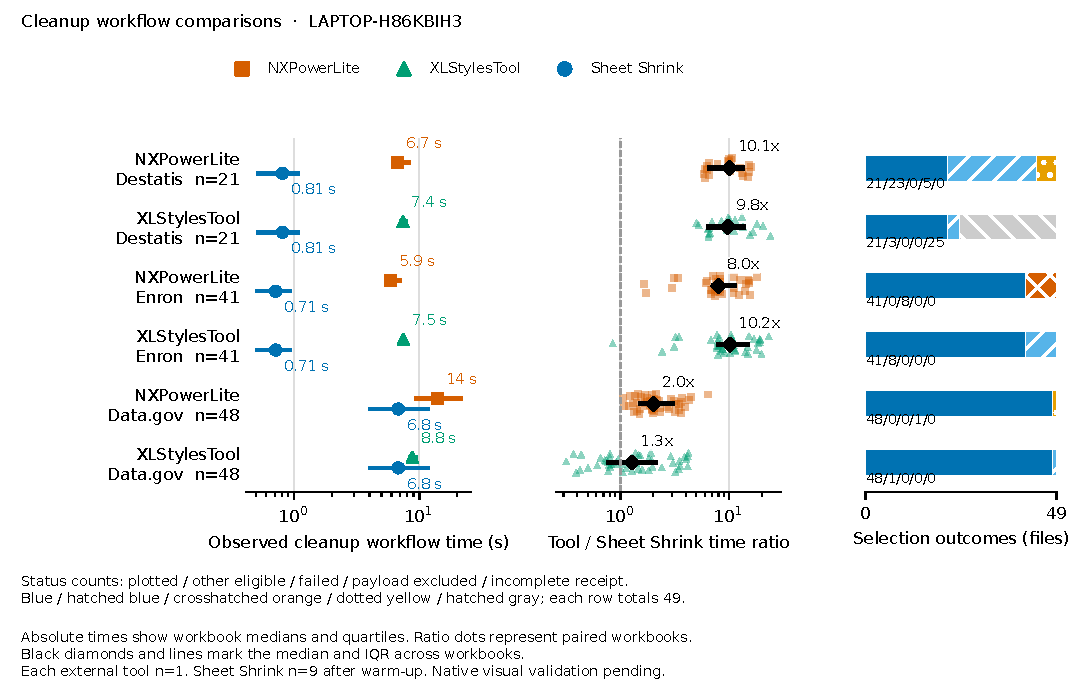
\includegraphics[width=\columnwidth]{figures/paired-cleanup-workflows.pdf}
\caption{Cleanup times and tool/SheetShrink ratios by corpus; parentheses give
pair counts. Time summaries and black ratio marks show medians and interquartile
ranges. NXPL: NXPowerLite; XLST: XLStylesTool; CP: Check Performance; INQ: Inquire.}
\label{fig:paired-cleanup-workflows}
\end{figure}


\subsection{Native validation of preservation rules}
\paragraph{Row-height preservation.}
In the Traffic workbook, promoting repeated empty-cell formatting into a row style
changed an automatically determined height from 12.75 to 9 points, shifting
subsequent content and changing 3,408 pixels in an independently specified reference
region. Requiring an explicit custom height before promotion restored byte-identical
native captures~\cite{rowpromotionfix}.

\paragraph{Font representatives.}
Two Destatis cases validate complementary font-preservation conditions. In a
higher-education workbook, removing 87 blank cells carrying explicit default-font and
no-fill metadata changed 25,640 pixels despite equal capture geometry and a
pixel-identical original-versus-original control. Retaining the required
representatives restored equality in an independently specified reference region.
Legacy print-name aliases were normalized for opening and recorded separately. In a
cultural-finance workbook, a blank cell's non-default font affected automatic row
height despite an omitted \texttt{applyFont} flag; a stored height without
\texttt{customHeight} did not prevent the change from 15 to 12.75 points. Retaining
the representative restored pixel and geometry equality in the independent control
and all 350 regions selected by the targeted capture policy.

\paragraph{Background definitions.}
In a Destatis horticulture workbook, SheetShrink reduced column definitions from
128,912 to 2,197. A corrected DeltaSieve background-envelope guard reduced the
capture selection from 16,101 to 165 regions; all 165 resulting image pairs were
pixel-identical.

\paragraph{Validation boundaries.}
In Wanderungen, excluding an empty trailing context row removed a spurious height
finding. All 37 captured image pairs were pixel-identical under the DeltaSieve
capture policy, while separate effective-height observations on two other worksheets
remained unresolved~\cite{trailingrowvalidation}.
These case studies validate specific preservation conditions within the recorded
capture scopes; they do not establish exhaustive workbook or corpus-wide visual
equivalence.

\subsection{Targeted visual outcomes on the Top49 selection}
A version-matched audit of the 49 workbooks with the largest absolute
SheetShrink reductions in each corpus retained 42 Destatis, 46 Data.gov,
and 46 Enron comparisons against the selected originals. Separately
documented normalized baselines supplied five further Destatis and two
further Enron observations. The remaining two, three, and one slots,
respectively, had no eligible observation. Across both baseline categories,
zero Destatis, seven Data.gov, and five Enron workbooks had recorded
differences. These counts describe the selected capture scope and include
findings whose cause remains unresolved. The five Enron workbooks had six
chart findings of 2--26 changed pixels with equal image dimensions and no
reported geometry change. The missing Enron workbook required repair
when opened in Excel, including after a separate legacy reconversion.

\subsection{Evidence boundary}
The selected controls demonstrate concrete preservation conditions and recorded
failures. They do not estimate corpus-wide defect prevalence. Reduction results
cover the frozen XLSX inventories. Matched cleanup-plus-opening measurements and
independent native references cover selected cases. Broader reference coverage
and matched whole-corpus cost remain open. Detailed development attempts, input hashes, native images and
producer versions remain in the source-linked artifact.
